\title{Střední Evropa}
\documentclass[10pt,a4paper]{article}
\usepackage[utf8]{inputenc}
\usepackage[czech]{babel}
\usepackage{amsmath}
\usepackage{amsfonts}
\usepackage{amssymb}
\usepackage{chemfig}
\usepackage{geometry}
\usepackage{wrapfig}
\usepackage{graphicx}
\usepackage{floatflt}
\usepackage{hyperref}
\usepackage{fancyhdr}
\usepackage{tabularx}
\usepackage{makecell}
\usepackage{csquotes}
\usepackage{footnote}
\usepackage{movie15}
\MakeOuterQuote{"}

\renewcommand{\labelitemii}{$\circ$}
\renewcommand{\labelitemiii}{--}
\newcommand{\ra}{$\rightarrow$ }
\newcommand{\x}{$\times$ }
\newcommand{\lp}[2]{#1 -- #2}
\newcommand{\timeline}{\input{timeline}}


\geometry{lmargin = 0.8in, rmargin = 0.8in, tmargin = 0.8in, bmargin = 0.8in}
\date{\today}
\author{Jakub Rádl}

\makeatletter
\let\thetitle\@title
\let\theauthor\@author
\makeatother

\hypersetup{
colorlinks=true,
linkcolor=black,
urlcolor=cyan,
}



\begin{document}
\maketitle
\tableofcontents
\begin{figure}[b]
Toto dílo \textit{\thetitle} podléhá licenci Creative Commons \href{https://creativecommons.org/licenses/by-nc/4.0/}{CC BY-NC 4.0}.\\ (creativecommons.org/licenses/by-nc/4.0/)
\end{figure}
\newpage

\mbox{}
\vspace{-1.5cm}
\begin{wrapfigure}{r}{3cm}
\frame{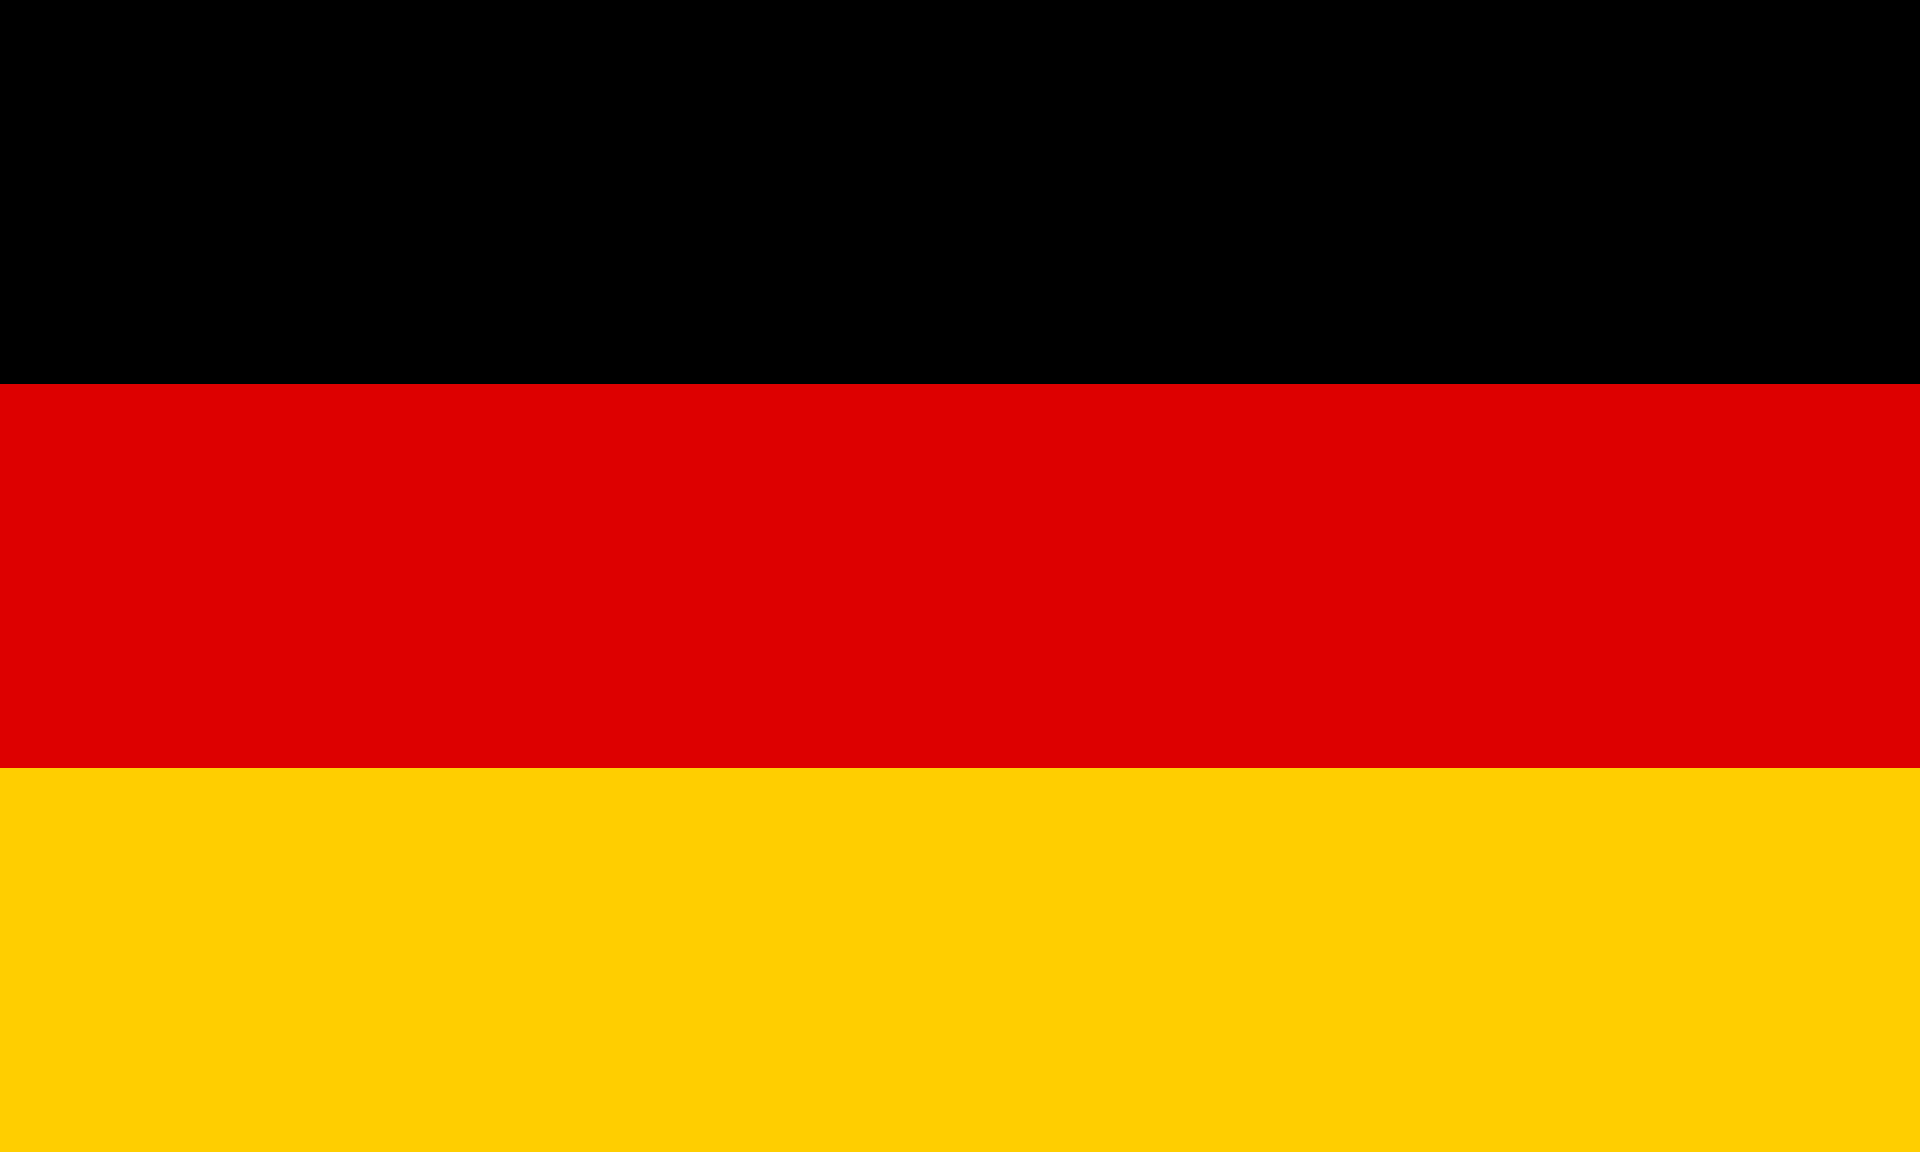
\includegraphics[height=2cm]{pictures/flag_DE.png}}
\vspace{-200pt}
\end{wrapfigure}
\section{Německo}



\newpage
\mbox{}
\vspace{-1.5cm}
\begin{wrapfigure}{r}{3cm}
\frame{
\includegraphics[height=2cm]{pictures/flag_A.png}}
\vspace{-200pt}
\end{wrapfigure}
\section{Rakousko}



\newpage
\mbox{}
\vspace{-1.5cm}
\begin{wrapfigure}{r}{3cm}
\frame{
\includegraphics[height=2cm]{pictures/flag_CH.png}}
\vspace{-200pt}
\end{wrapfigure}
\section{Švýcarsko}



\newpage
\mbox{}
\vspace{-1.5cm}
\begin{wrapfigure}{r}{3cm}
\frame{
\includegraphics[height=2cm]{pictures/flag_PL.png}}
\vspace{-200pt}
\end{wrapfigure}
\section{Polsko}
\subsection{Přírodní podmínky}
\paragraph{Otázečky}
\begin{enumerate}
\item Vyhledej na mapě: Pomořanská, Mazurská jezerní plošina; Velkopolská, Slezská, Mazovská nížina; Lublinská, Malopolská vrchovina; pohraniční pohoří s Českem a Slovenskem; Bělověřský prales; řeky Visla, Odra, Varta; jezero Sinardwy
\end{enumerate}

\paragraph{Povrch}
\begin{itemize}
\item většina povrchu -- \textbf{nížiny} a ledovcové \textbf{jezerní plošiny}
\item v jižní části vrchoviny, na hranici s ČR a SR pohoří
\item nížiny kolem Baltského moře ( ... )
\item přechod kontinentálního klimatu od severu k jihu
\end{itemize}

\paragraph{Vodstvo}
\begin{itemize}
\item většina řek je odvodňována do \textbf{Baltského moře}
\item \textbf{Sinardwy} -- největší jezero, v Mazurské plošině
\item \textbf{Helská kosa} (kosa = pruh pevniny nanesený mořskými proudy)
\end{itemize}

\paragraph{Běloveský národní park}
\begin{itemize}
\item na Hranici s Běloruskem
\item populace \textbf{zubra evropského}, divokých koňů (tarpanů)
\item nížinný typ pralesa s převahou listnatých dřevin (staleté duby)
\end{itemize}

\paragraph{Sloviňský národní park}
\begin{itemize}
\item na pobřeží Baltu
\item pohyblivé \textbf{písečné duny}
\item jezera občas sycená mořskou vodou (při bouřích) \ra výskyt \textbf{halofytních} (slanomilných) druhů (los, bobr, tuleň, sviňucha)
\end{itemize}


\subsection{Historie, obyvatelstvo, administrativní členění}
\paragraph{Otázečky}
\begin{enumerate}
\item Na mapách v atlase (\textit{str. 52, 53}) a pomocí textu v učebnici (\textit{str. 32}) vyhodnoť územní změny v Polsku
\end{enumerate}

\paragraph{Historie}
\begin{itemize}
\item polsko-litevské knížectví
\item německá kolonizace severu a západu
\item trojí dělení Polska
\item změna hranic po 2. sv. válce
\item Varšava po 2. sv. válce zničena (v nedávné době obnovena)
\item vyvraždění důstojníků polské armády Sověty
\end{itemize}

\paragraph{Obyvatelstvo}
\begin{itemize}
\item 38 milionů obyvatel
\item husté osídlení jihu v pásu od Wroclavi po Katovice (výskyt surovin $\rightarrow$ průmysl)
\item k hlavním centrům patří Vršava, Poznaň, Lódž, Vroclav, Katovice, Krakov, Gdaňsk, Štětín
\item \textbf{rozdíly v životní úrovni} ve městech a na venkově
\item rozdíly mezi vyspělostí západu a východu
\end{itemize}

\paragraph{Administrativní členění}
\begin{itemize}
\item členěno na \textbf{vojvodství} (ekvivalent českých krajů)
\end{itemize}

\paragraph{Významná města}
\begin{itemize}
\item \textbf{Gdaňsk} -- přístav
\item \textbf{Malbork} -- křižácká pevnost
\item \textbf{Krakov} -- ve své době sídlem králů, hrad Wawel
\item \textbf{Lešno} -- shořely zde spisy J. A. Komenského
\item \textbf{Toruň} -- rodiště Mikoláše Koperníka (autor heliocentrického světového názoru)
\item \textbf{Osvětim-Březinka} -- koncentrační tábor
\item \textbf{Wieliczka} -- solné doly (těžba ukončena, ze soli vytesané sochy)
\item \textbf{Zakopane} -- lyžařské středisko
\end{itemize}


\subsection{Ekonomika}
\begin{itemize}
\item člen EU
\item zásoby \textbf{surovin} na jihu (uhlí, síra, zinek, měď)
\item průmysl soustředěný v oblasti \textbf{Horno a Dolnoslezské pánve}
\item těžba a průmysl se projevuje na životním prostředí $\rightarrow$\textbf{ útlum a restrukturalizace} těžkého průmyslu
\end{itemize}

\paragraph{Zemědělství}
\begin{itemize}
\item velká zemědělská produkce
\item stále \textbf{vysoký podíl pracujících v zemědělství} (cca 12%)
\item významná \textbf{produkce žita, lnu, brambor, cukrové řepy a masa}
\end{itemize}

\paragraph{Katovická aglomerace (konurbace)}
\begin{itemize}
\item \textbf{největší} aglomerace ve \textbf{východní části střední Evropy}
\item problémy s útlumem těžkého průmyslu
\item města: Katovice, Sosnowiec, Gliwice, Chorzow
\item největší síť tramvajové dopravy na světě (spojuje města)
\end{itemize}



\newpage
\mbox{}
\vspace{-1.5cm}
\begin{wrapfigure}{r}{3cm}
\frame{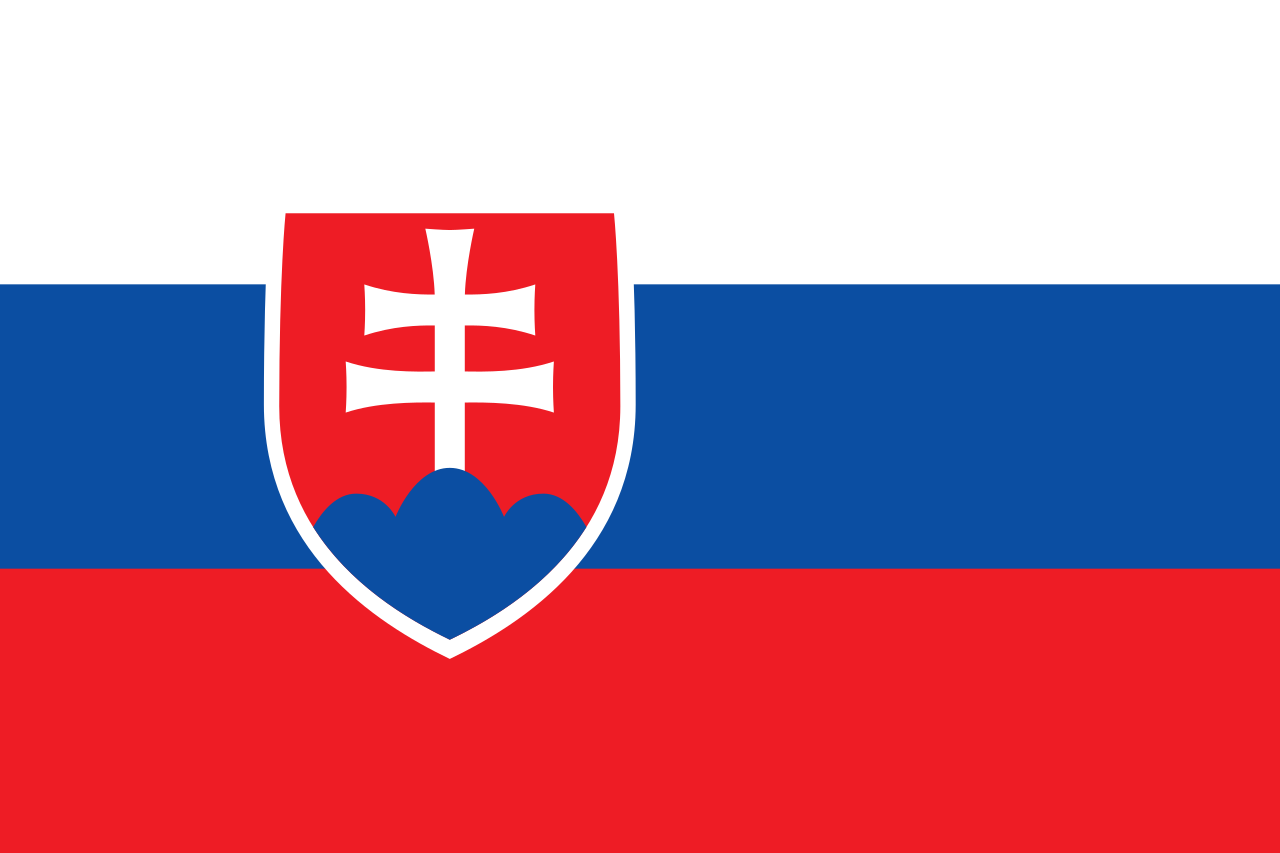
\includegraphics[height=2cm]{pictures/flag_SK.png}}
\vspace{-200pt}
\end{wrapfigure}	
\section{Slovensko} 
\subsection{Karpatský oblouk}
\begin{itemize}
\item pásemné pohoří táhnoucí se cca \textbf{1500km}
\item táhne se přes konec Rakouska, bok ČR, \textbf{Slovensko}, jih Polska, \textbf{Ukrajinu}, \textbf{Rumunsko}, sever Srbska
\item v pleistocénu zalednění nejvyšších oblastí, dnes jen pozůstalé ledovcové útvary
\item dělení
\begin{itemize}
\item Západní (\textbf{Gerlachovský štít} -- 2655, Slovensko)
\item Východní (\textbf{Pietrosul} -- 2303, Rumunsko)
\item Jižní (\textbf{Moldoveanu} -- 2543, Ukrajina)
\end{itemize}
\item horninový poklad tvořen flyšovým pásmem (pískovce, břidlice), krystalickými horninami (žula), vápenci a vulkanickými horninami
\begin{itemize}
\item vnější Karpaty -- pískovce, břidlice
\item vnitřní Karpaty -- pevné krystalické horniny
\end{itemize}
\item rozsáhlé plochy lesních porostů, velká populace vlků a medvědů
\end{itemize}


\subsection{Přírodní podmínky}
\begin{itemize}
\item většinu území zabírají \textbf{Karpaty} (flyšové a centrální pásmo -- vnější a vnitřní západní Karpaty)
\item nejvyšší pohoří
\begin{itemize}
\item \textbf{Tatry} (\textbf{Gerlachovský štít} -- 2655)
\item \textbf{Nízké Tatry} (\textbf{Ďumbier} -- 2043, Chopok)
\end{itemize}
\item třetí nejzalesněnější stát Evropy
\item soustava horských kotlin -- Liptovská + Popradská (Podtatranská), Turčianská (mezi Malou a Velkou Fatrou), Horehronská
\item množství národních parků (TANAP, NAPANT, Pieniny, Malá Fatra, Slovenský kras)
\item výběžky Panonské pánve -- Podunajská a Východoslovenská nížina
\item řeky Dunaj, Váh, Nitra, Hron (všechny na jihozápadě vtékají do Dunaje)
\begin{itemize}
\item \textbf{Dunaj}
\begin{itemize}
\item velké říční přístavy v Bratislavě a Komárně
\item Malý Dunaj -- rameno Dunaje odpojující se v Bratislavě a vracející se v Komárně
\item přehrada Gabčíkovo
\end{itemize}
\item \textbf{Váh}
\end{itemize}
\end{itemize}


\paragraph{Tatry}
\begin{itemize}
\item nejvyšší pohoří Slovenska a Karpat
\item rozdělení na \textbf{Západní} (Roháče), \textbf{Východní} (Vysoké a Belanské)
\item jsou součástí TANAPu, který je v seznamu UNESCO
\item nejznámější vrcholy: Gerlach, Kriváň, Vysoká, Lomnický štít, Rysy, Slavkovský štít
\item pramen Bieleho Váhu
\item od Nízkých Tater je pohoří odděleno Podtatranskou kotlinou s Liptovskou Mašou
\end{itemize}

\paragraph{Pieniny}
\begin{itemize}
\item \textbf{národní park} na hranici Slovenska s Polskem
\item pohoří tvořeno převážně jurskými a křídovými \textbf{vápenci}
\item hluboké \textbf{údolí a soutěsky} vymodelované řekou \textbf{Dunajec}
\item vrchol \textbf{Trzy Korony} s pěti skalními věžemi (až 100m)
\item vodáctví na Dunajci
\begin{itemize}
\item \textbf{pltě} -- dřevěné rafty
\end{itemize}
\end{itemize}

\paragraph{Slovenský kras}
\begin{itemize}
\item největší krasové území na Slovensku ($>$ 400 km$^2$), UNESCO
\item rozkládá se na hranici s Maďarskem
\item náhorní planiny, závrty, propasti, jeskyně, \ldots
\item jeskyně \textbf{Domica}
\begin{itemize}
\item státní hranice
\item největší známý stalagmit na světě (25m)
\end{itemize}
\end{itemize}


\subsection{Historie, sociální prostředí}
\paragraph{Otázečky}
\begin{enumerate}
\item Vyhledej v atlase: Košice, Žilina, Poprad, Banská Bystrica, Trenčín, Trnava, Nitra, Zvolen, Banská Šťiavnica, Vlkolínec, Bardejov, Spišský hrad
\item Seznamte se s administrativním členěním Slovenska
\end{enumerate}

\paragraph{Historie}
\begin{itemize}
\item 900 let součástí \textbf{uher}
\item 1918 -- vznik \textbf{Československa}
\item vyhlášení \textbf{Slovenského štátu} 1939-1945 (část dnešního území Slovenska pod nadvládou Maďarska)
\item 1993 -- \textbf{Slovenská republika}
\end{itemize}

\paragraph{Sociální prostředí}
\begin{itemize}
\item \textbf{nerovnoměrné rozmístění obyvatelstva} v důsledku horského reliéfu
\item soustředění obyvatelstva v \textbf{Podunajské nížině}
\item excentrická poloha Bratislavy (po rozpadu návrhy Banské Bystrice jako hlavního města)
\item 10\%\textbf{ maďarská menšina}
\item administrativní dělení na \textbf{kraje}
\end{itemize}


\paragraph{Zajímavosti}
\begin{itemize}
\item torzo hradu \textbf{Děvín} na soutoku Moravy a Dunaje (bývalé hradiště)
\item \textbf{Bratislavský hrad} (nesídlí zde prezident)
\item \textbf{Nový most} v Bratislavě (přes Dunaj, původně Most slovenského národního povstání)
\item \textbf{Michalská brána} v Bratislavě
\item \textbf{Vlkolínec} -- podhorská vesnička (poblíž Ružomberoku)
\item \textbf{Spišský hrad} (UNESCO), východně od Nízkých Tater
\item \textbf{Banská Štiavnica} -- poblíž Bystrice, dříve těžba, historické jádro (UNESCO)
\item historická část města \textbf{Bardějov} (UNESCO), severovýchod
\end{itemize}

\subsection{Ekonomika Slovenska}
\paragraph{Historie}
\begin{itemize}
\item stagnace za nadvlády Maďarů
\item slabý rozvoj v prvorepublikovém období Československa
\item \textbf{industrializace} po 2. sv. válce s důrazem na \textbf{těžký průmysl}
	\begin{itemize}
	\item nutnost dovozu surovin
	\item poškození životního prostředí
	\item v současnosti probíhá \textbf{restrukturalizace}
	\end{itemize}
\item po\textbf{ rozpadu Československa}
	\begin{itemize}
	\item oslabení pozic na rozpadajících se východních trzích
	\item \textbf{ekonomické reformy} s negativním vlivem na obyvatelstvo (později s ekonomickými pozitivy)
	\end{itemize}
\item 2004 -- vstup do \textbf{EU}
	\begin{itemize}
	\item otevření přístupu na \textbf{evropské trhy}	
	\item příliv \textbf{zahraničního kapitálu} (investice do např. automobilového průmyslu)
	\item příliv \textbf{zahraniční konkurence}
	\end{itemize}
\end{itemize}

\paragraph{Průmysl}
\begin{itemize}
\item soustředěný v \textbf{Pováží}, \textbf{Bratislavě}, \textbf{Košicích} a menších regionálních centrech (Banská Bystrica, Trnava, Poprad)
\item výroba \textbf{automobilů}: Volkswagen, Peugeot, Citroen, Kia (nová pracovní místa)
\item \textbf{elektrotechnický průmysl}
\item Slovnaft Bratislava (ropovod z Ruska)
\end{itemize}

\paragraph{Zemědělství}
\begin{itemize}
\item využití \textbf{Podunajské nížiny}
\item hospodaření v horských oblastech podobné alpskému zemědělství 
\end{itemize}

\paragraph{Dopravní síť}
\begin{itemize}
\item \textbf{nutnost modernizace} (nedostavěné dálnice, rychlostní železnice)
\item dobré perspektivy v oblasti cestovního ruchu
\item nedokončená dálnice D1 přes sever Slovenska (Trenčín, Ružomberok, Poprad, Prešov)
\item v jižní části dálnice chybí
\end{itemize}



\newpage
\mbox{}
\vspace{-1.5cm}
\begin{wrapfigure}{r}{4cm}
\frame{
\includegraphics[height=2cm]{pictures/flag_HU.png}}
\vspace{-50pt}
\end{wrapfigure}	
\section{Maďarsko}
\subsection{Přírodní podmínky}
\begin{enumerate}
\item Vyhledej na mapě: Velká a Malá uherská nížina; Bakoňský les, Mátra, Bukové hory, Tisza, Balaton; NP Hortobágy
\item Zjisti z atlasu typ klimatu příznačný pro Maďarsko
\item Jaké půdy a jaký rostlinný pás převažují na území Maďarska
\end{enumerate}

\paragraph{Povrch}
\begin{itemize}
\item většina Maďarska -- \textbf{nížiny} (Velká uherská, Malá uherská)
\item na severu pohoří Mátra (Kékes, 1015)
\item na severovýchodě řeka \textbf{Rába}, na jihu \textbf{Dráva}, na východě\textbf{ Tisza}
\end{itemize}


\paragraph{Panonská pánev}
\begin{itemize}
\item \textbf{puszta} (pusta) = step
\item rozsáhlá deprese rozkládající se především na území Maďarska a okrajově zasahující do sousedních států.
\item ve třetihorách moře
\item pokryta silnou vrstvou mořských, říčních a eolických (větrných) \textbf{usazenin}
\item bohaté zásoby podzemních vod v nánosech
\item původní stepi byly většinou přeměněny na zemědělskou krajinu
\item zbytky pusty jsou zachovány v NP Hortobágy
\end{itemize}

\paragraph{NP Hortobágy}
\begin{itemize}
\item severovýchod Maďarska, 700km$^2$
\item tvořen \textbf{pustou, rybníky a močály}
\item rozsáhlé pastviny, vodní plochy s bažinami \ra \textbf{mnoho ptáků} (racek chechtavý, volavka červená, bílá)
\item na stepi se pasou stáda skotu, ovcí a polodivokých koní
\item v centru parku se nachází vesnice Hortobágy
	\begin{itemize}
	\item Velkoá csárda (zájezdní hostinec)
	\item nejdelší kamenný Most v Maďarsku (170m)
	\end{itemize}
\item biosférická rezervace na seznamu \textbf{UNESCO}
\end{itemize}

\paragraph{Blatenské jezero - "Balaton"}
\begin{itemize}
\item \textbf{největší jezero ve střední Evropě}, tektonického původu o rozloze 596km$^2$
\item pobřeží je strmé, zbylé oblasti jsou ploché a bažinaté, mělké (11m), vysychá
\item v jižní části významná hnízdiště ptactva
\item zanášeno \textbf{usazeninami} (nanesenými větrem) \ra nutno bagrovat
\item nejdůležitější \textbf{lázeňská oblast}, po Budapešti druhé nejnavštěvovanější místo v Maďarsku
\end{itemize}

\paragraph{Termální vody}
\begin{itemize}
\item vyskytují se na 60\% území a využívají se v lázeňství, k vytápění bytů nebo skleníků
\item mezi vyhlášené lázně patří také Budapešť, kde byly termální vody známé již ve starověku
\end{itemize}

\subsection{Historie, obyvatelstvo, sídla}
\paragraph{Historie}
\begin{itemize}
\item ve starověku římská provincie Panonie
\item v 9. stol. příchod Maďarů do Evropy od Uralu
\item 1526 -- bitva u Moháče (jih Maďarska) \ra Maďarsko součástí Habsburské monarchie
\item 1867 -- rakousko-uherské vyrovnání
\item po rozpadu monarchie ztráta $\frac{2}{3}$ území
\item role Maďarska za 2. sv. války
	\begin{itemize}
	\item oficiální spojenci německa \ra poražená země
	\end{itemize}
	\item 1956 -- revoluce
\end{itemize}

\paragraph{Obyvatelstvo}
\begin{itemize}
\item národnostně \textbf{homogenní} stát
\item maďarské \textbf{menšiny v sousedních zemích}
\item maďarština patří k ugrofinským jazykům
\end{itemize}

\paragraph{Sídla}
\begin{itemize}
\item dominantní role Budapešti a posilování vlivu menších regionálních center (Miskolc, Debrecen, Pécs, Györ)
\item velké vesnice a množství samot
\item administrativní členění na \textbf{župy}
\end{itemize}

\paragraph{Budapešť}
\begin{itemize}
\item římský vojenský tábor a osada Aquincum na místě dnešní Budapešťi
\item po příchodu Maďarů dvě osady Buda, Pešť
\item po roce 1526 města obsazena Turky (hlavním městem Uher se stává Prešpurk 1536--1784)
\item 2. pol. 19. stol. spojení obou měst -- Budapešť
\item královský palác -- Budínský hrad
\item Matyášův chrám (gotický)
\item Rybářská bašta
\item řetězový most
\item parlament
\item metro -- nejstarší na Evropském kontinentě (1896) (Londýn má starší)
\item termální lázně 
\end{itemize}

\subsection{Ekonomika Maďarska}
\begin{itemize}
\item intenzivní zemědělství zaměřené na produkci obilovin, ovoce, zeleniny, vinné révy (Tokaj), chov prasat a skotu
\item export \textbf{potravinářských výrobků}: vepřové maso, čabajka, uherák, víno, mletá paprika
\item z nerostných surovin má význam pouze těžba bauxitu
\item rozvinutý průmysl \textbf{elektrotechnický, dopravní, potravinářský, farmaceutický}
\item hospodářský jádrem země je \textbf{budapešťská aglomerace}
\end{itemize}



\newpage
\mbox{}
\vspace{-1.5cm}
\begin{wrapfigure}{r}{4cm}
\frame{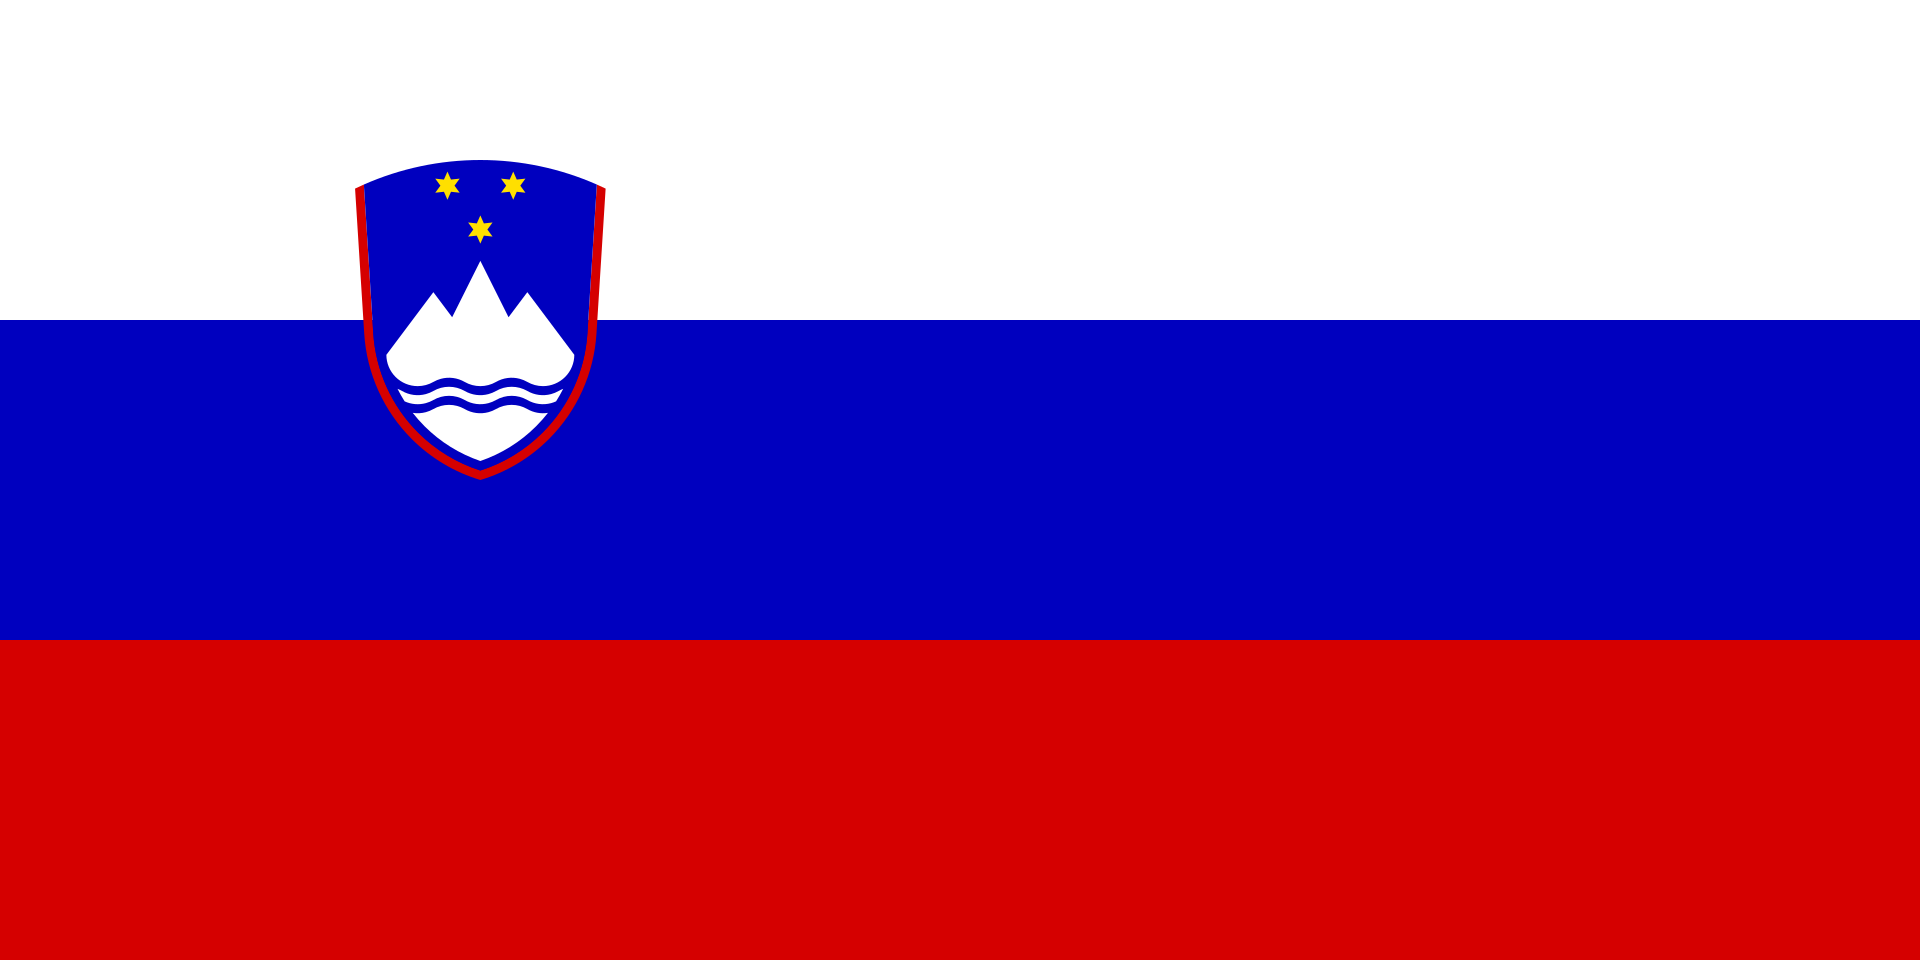
\includegraphics[height=2cm]{pictures/flag_SLO.png}}
\vspace{-50pt}
\end{wrapfigure}	
\section{Slovinsko}
\subsection{Celková charakteristika státu}
\begin{itemize}
\item v minulosti součást rakouské monarchie
\item po 1. sv. válce vznik Jugoslávie
\item po 2. sv. válce se Slovinsko stává nejvyspělejší zemí v regionu
\item v roce 1991 zisk samostatnosti
\item výroba sportovních potřeb (Lyže Elan)
\item \textbf{farmaceutický} průmysl (soustředěný okolo řeky Krka)
\item dobré podmínky v oblasti cestovního ruchu
\item \textbf{tranzitní poloha}
\end{itemize}

\paragraph{Zajímavosti}
\begin{itemize}
\item \textbf{Triglav} -- nejvyšší vrchol (2052), na vlajce 
\item krasové oblasti -- \textbf{Postojna jeskyně}
\item Julské Alpy
\item \textbf{Planica} -- světový pohár skoku na lyžích
\item \textbf{Kranjska Gora} -- světový pohár ve sjezdovém lyžování
\item horolezectví, canyoning, sjíždění divokých řek, horská cyklistika
\item jezero \textbf{Bled} -- mezinárodní závody ve veslování
\end{itemize}





\end{document}
